
\section{Signal Corrections in the LUX Detector} \label{StandardCalibrations}

In this chapter, we discuss the need for position dependent corrections to the S1 and S2 signals in LUX.  Position dependence in the S1 signal can be introduced by a number of effects.  As photons travel from an interaction site to the PMT arrays they are reflected by teflon panels surrounding the active volume.  The amount of reflected light varies based on the proximity of the event to the teflon walls, the angle of incidence of the light, and the surface properties of the teflon.   Photons are also reflected and refracted at the liquid xenon surface, causing about two thirds of the S1 signal to be collected in the bottom PMT array.  Events which are closer to the bottom have more solid angle covered by the bottom PMT array, leading to a larger S1 collection.  A z-dependence of the light collection efficiency can also be introduced by light quenching impurities present in the liquid xenon, although this effect is negligible at the liquid xenon purity levels found in LUX.

As electrons travel from the interaction site to the liquid surface they are absorbed by electronegative impurities in the liquid xenon.  This attenuation of charge leads to a smaller S2 signals from events originating deeper in the detector.  Since the purity of the liquid xenon changes on a weekly basis, there is a significant time dependence in the strength of this effect. Small changes in the X-Y plane of the extraction field or the liquid surface level can lead to a position dependence in both the efficiency at which electrons are extracted from the liquid xenon, and the number of photoelectrons which are produced per extracted electrons.  Both of these effects are reflected in the size of the S2 signal.  Furthermore, while the individual PMTs are gain matched with LED calibrations, the variation in quantum efficiency between PMTs can lead to an X-Y position dependence in both the S1 and S2 signals.

In the final data analysis, we wish to know the average number of photons and electrons produced by recoil interactions of both types, as well as the fluctuations around those averages.  It is possible to define position dependent gain factors which convert the S1 signals and S2 signals to number of photons and number of electrons, respectively, but it is more convenient to normalize the S1 and S2 signals to one location in the detector.   Likewise, one could define position and time dependent ER and NR bands to track discrimination over time, but it is more convenient to normalize the data such that the ER band and NR bands are constant at all times and all locations in the detector.  In LUX we choose to normalize the S1 signal to the center of the detector, and the S2 signal to the top of the detector.  The choice to normalize the S1 signal to the center of the detector is arbitrary since the position dependence of the S1 signal has little time dependence, while the choice to normalize the S2 signal to the top of the detector is convenient for circumventing the time dependence inherent at deeper locations in the detector due to varying amount of electron absorbing impurities in the liquid xenon.  Once the S1 and S2 signals are uniform throughout the detector we can define one position independent gain factor for each of the detector signals.  Removing the position dependence of the S1 and S2 signals also results in increased energy resolution of the S1 and S2 spectra, as well as a narrowing of the ER and NR band widths.


Note that a non-uniform drift field can also introduce position dependence to the S1 and S2 signals.  However, this effect changes the actual number of photons and electrons produced during a recoil interaction, rather than the detector's efficiency of collecting those photons and electrons.  In this chapter we will assume a uniform drift field is present in the detector, as was generally the case in LUX Run3 when the field varried by less than 8\%. We will discuss signal corrections for a detector with a nonuniform electric field in Chapter~\ref{Run04Corrections}.

\subsection{Use of $^{83m}$Kr in Signal Corrections} \label{KrSource}

The LUX detector's $^{83m}$Kr calibration source is a powerful tool to measure corrections for the S1 and S2 signals. A $^{83}$Rb soaked charcoal source is used to inject its $^{83m}$Kr daughter directly into the LUX circulation system.  In the active volume the $^{83m}$Kr decays via internal conversion at 32.1 keV and 9.4 keV with a half life of 1.86 hours (Figure~\ref{KrDecayScheme}).  The half life of the 9.4 keV decay is only 154 ns, causing the two decays to merge into one 41.55 keV pulse in the LUX detector.  Note that it is possible to modify the LUX pulse finder to separate the two S1 signals when desired, but it is nearly impossible to separate the two S2 signals due to diffusion of the electron clouds as they drift to the liquid surface, and the relatively long width of the S2 pulse as the electrons transit the gas phase.

\begin{figure} [!h]
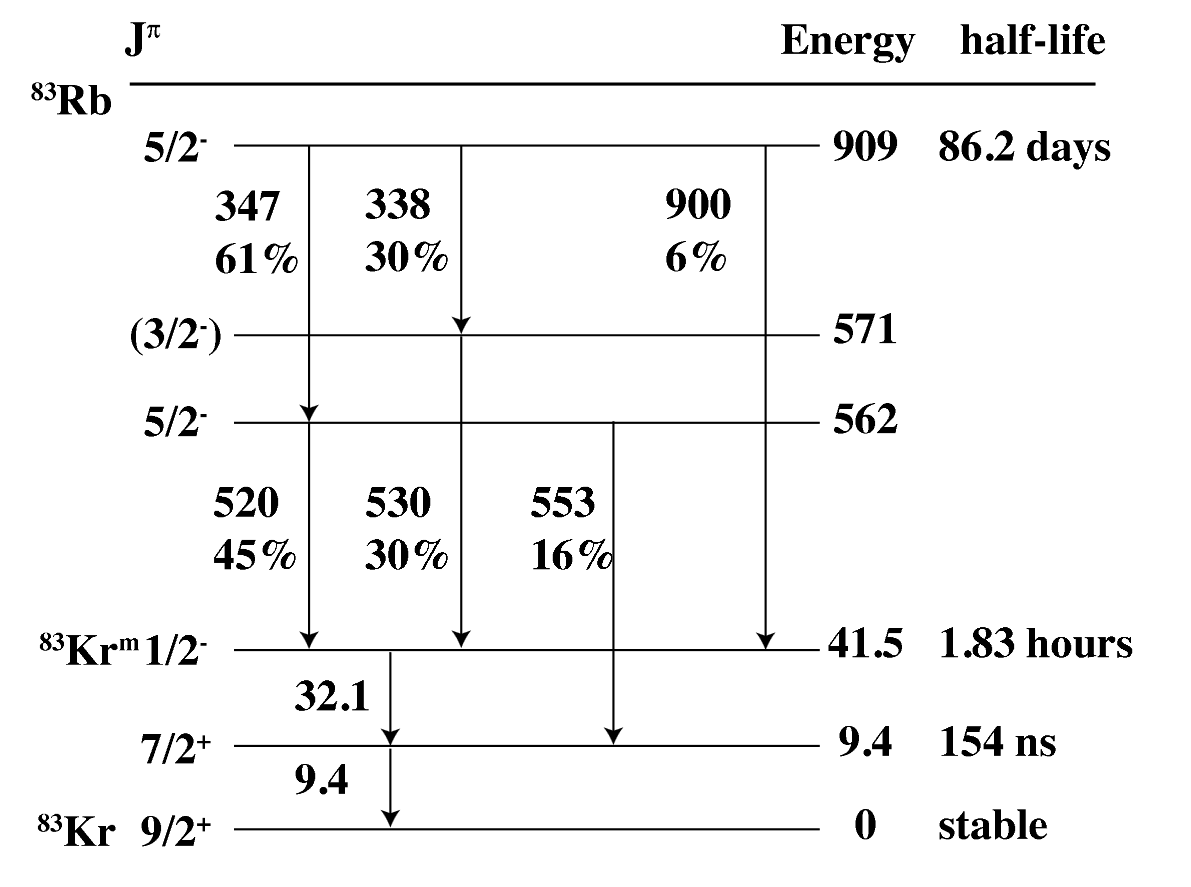
\includegraphics[scale=.35]{Kr83Decay.png} 
\captionof{figure}{The energy level diagram of the $^{83}$Rb and $^{83m}$Kr decays.}
\label{KrDecayScheme}
\end{figure}

Once injected, the $^{83m}$Kr mixes uniformly throughout the active volume in a matter of minutes (Figure~\ref{fig:KrMixing}). The monoenergetic peak of the $^{83m}$Kr events can be measured at any point in the detector to determine the position dependence of the S1 and S2 signals.

\begin{figure} 
\centering
\subfloat{{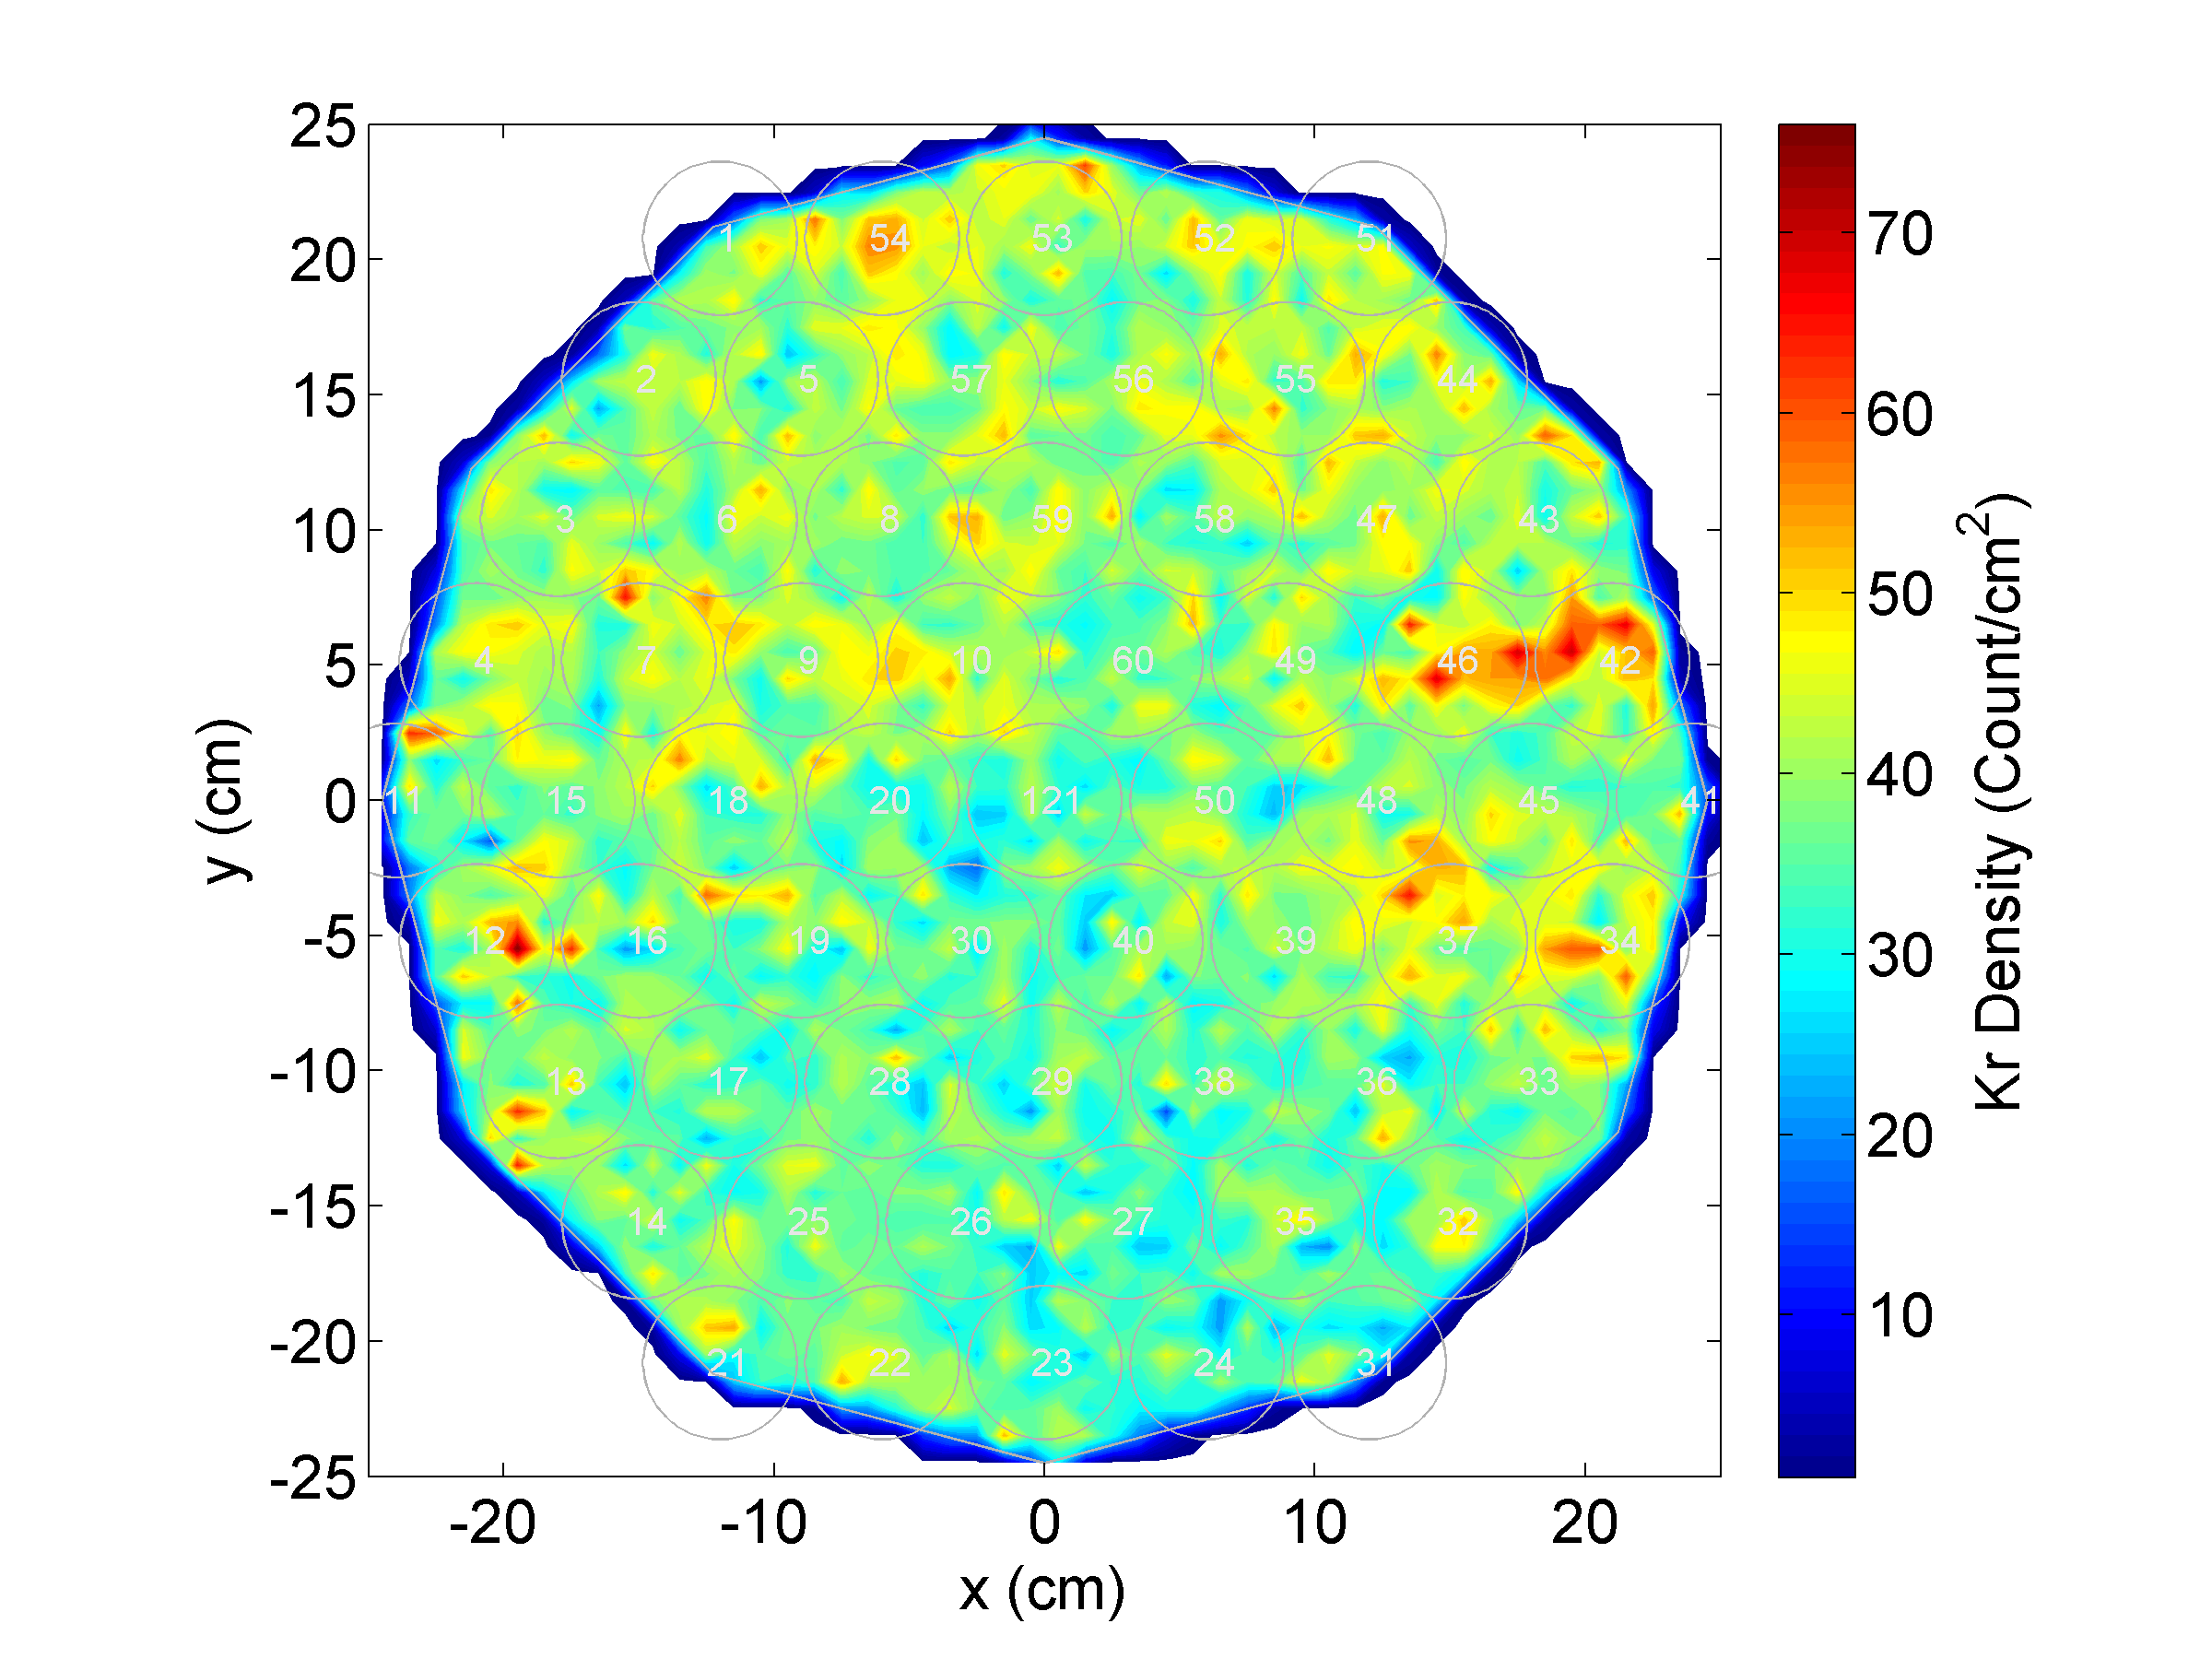
\includegraphics[width=6cm]{KrXvY.png} }}
\qquad
\subfloat{{\includegraphics[width=6cm]{KrR2vz.png} }}
\caption{ (Left) Density of $^{83m}$Kr events in the X-Y plane 10-30 minutes after a $^{83m}$Kr injection. (Right) Density of $^{83m}$Kr events in the R$^2$-Z plane 10-30 minutes after a $^{83m}$Kr injection.  Data from lux10\_20130510T1250. }
\label{fig:KrMixing}
\end{figure}
%Show R^2vZ and XY density plots of Kr for high stats injection in 2015 with time cut of 10-30 minutes to show quick mixing.

The short half life causes the calibration source to be removed from the LUX detector in a matter of hours, allowing for calibration of the S1 and S2 signals on a weekly basis.  This is a crucial property of the calibration source, since the purity of the liquid xenon, and therefore the z-dependence of the S2 signal, changes on a weekly basis and we therefore wish to inject the source frequently.  It is also important that the $^{83m}$Kr is an inert noble gas, a property which prevents temporary attenuation of the S1 and S2 signals during injection of the calibration source. 


\subsection{S1 Corrections}\label{S1SignalCorr}

We first measure the Z dependence of the $^{83m}$Kr S1 pulse areas by slicing the detector into drift time bins with widths defined such that each bin has roughly 300 events, resulting in roughly 1 $\mu$second drift time bins.  A Gaussian distribution is fit to the S1 spectra of each bin to determine the location of the spectra means. A second order polynomial is used to determine the S1 Z dependence between and outside of each drift time bin (Figure~\ref{fig:KrypCal_S1ZDep}). A detector inefficiency correction for the Z direction is defined by taking the ratio of the S1  pulse area at the center of the detector (defined as $z_c$) to the S1 pulse area as a function of Z as described in the equation
\begin{equation}
\mbox{S}1_{\mbox{z-efficiency-correction}} = \frac{S1(z_c)}{S1(z)}.
\end{equation} 

%Show Run03 S1 gaussian fits and polynomial here -- can get it from the LUG probably
\begin{figure} 
\centering
\subfloat{{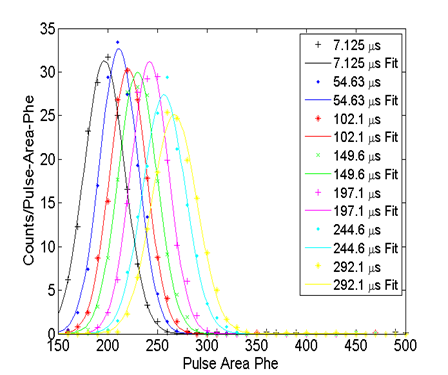
\includegraphics[width=6.3cm]{KrS1_ZDep_Gaussians.png} }}
\qquad
\subfloat{{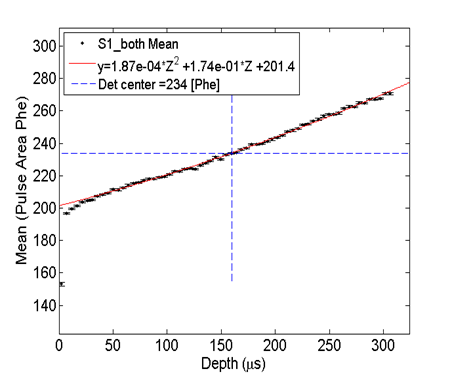
\includegraphics[width=6.3cm]{KrS1_ZDep.png} }}
\caption{ (Left) Gaussian distribution fits to $^{83m}$Kr S1 data that are used to determine the drift time dependence of the S1 pulse area. (Right) The z dependence of the S1 pulse area. Black points indicate the maximum of Gaussian distribution fits for each drift time bin, and red points indicate the polynomial fit to that data. Data from lux10\_20130510T1250.}
\label{fig:KrypCal_S1ZDep}
\end{figure}

The XY dependence of the S1 signal is found by dividing the z-corrected ($S1 \times \mbox{S}1_{\mbox{z-efficiency-correction}}$) data into two dimensional XY bins with dimensions defined such that each bin has roughly 300 events, typically resulting in $\sim$1.5 cm steps in each dimension.  A Gaussian distribution is fit to the data of each bin.  The mean of the Gaussian distribution from each bin is used to construct S1 XY response maps, with a spline interpolation and extrapolation being used to determine the XY dependence between and outside of the bins. (Figure~\ref{fig:KrypCalS1XYDep}) A detector inefficiency correction for the XY direction is defined by taking the ratio of the z-corrected S1 pulse area at the center of the detector to the z-corrected S1 pulse area as a function of XY in cm, as shown below
\begin{align}
\mbox{S}1_{\mbox{xy-efficiency-correction}} &= \frac{\mbox{S}1_{\mbox{z-efficiency-correction}}\times S1(x_c,y_c,z)}{\mbox{S}1_{\mbox{z-efficiency-correction}}\times S1(xyz)}.
\end{align} 
where $x_c$ and $y_c$ are the x and y center of the detector in uncorrected position coordinates. The corrected S1 pulse areas are produced by multiplying the raw, uncorrected S1 pulse areas by the XY and Z correction factors
\begin{equation}
\mbox{S}1_{\mbox{corrected}} = \mbox{S}1_{\mbox{raw}} \left( \mbox{S}1_{\mbox{z-efficiency-correction}} \right) \left( \mbox{S}1_{\mbox{xy-efficiency-correction}} \right).
\end{equation}

%Show S1 XY correction here
\begin{figure} 
\centering
\subfloat{{\includegraphics[width=6.3cm]{KrS1_XYDep.png} }}
\qquad
\subfloat{{\includegraphics[width=6.3cm]{KrS1_XYDep_Norm.png} }}
\caption{ (Left) Two dimensional map of the XY dependence in $^{83m}$Kr S1 data determined by fitting a Gaussian distribution to XY bins of the data and plotting the mean of each fit.(Right) Two dimensional map of the XY correction factor which is applied to z-corrected S1 data. Data from lux10\_20130510T1250.}
\label{fig:KrypCalS1XYDep}
\end{figure}


When over 300,000 events are present in a $^{83m}$Kr calibration data set, a three dimensional S1 corrections map is favored over the two step (Z, then XY) corrections described above.  In this case, the uncorrected S1 data is divided into three dimensional XYZ voxels with volumes defined such that each bin has roughly 300 events. A Gaussian distribution is fit to the data of each voxel, and the mean of the Gaussian distribution is used to construct three dimensional S1 dependence maps, with a spline interpolation and extrapolation being used to determine the XYZ dependence between and outside of the voxels. A three dimensional detector inefficiency correction is then defined by taking the ratio of the uncorrected S1 pulse area at the center of the detector to uncorrected S1 pulse area as a function of X,Y, and drift time, as shown below
\begin{align}
\mbox{S}1_{\mbox{xyz-efficiency-correction}} &= \frac{S1(x_c,y_c,z_c)}{S1(xyz)}.
\end{align} 
In this case, the corrected S1 pulse areas are produced by multiplying the raw, uncorrected S1 pulse areas by the XYZ correction factor.
\begin{equation}
\mbox{S}1_{\mbox{corrected}} = \mbox{S}1_{\mbox{raw}} \left( \mbox{S}1_{\mbox{xyz-efficiency-correction}} \right).
\end{equation}
The detector inefficiency effects in the S1 signal are due to the unchanging internal geometry of the detector, as well as the slowly changing PMT quantum efficiencies of the PMTs, which remain constant for many months.  Therefore, the S1 correction maps vary by only a few percent over time and a single high stats three dimensional correction map can be applied to data over a long period of time.  In the case of LUX Run3, the three dimensional S1 corrections map was only updated once, and each version was used for a span of roughly two months.

Figure~\ref{KrS1Improvement} show the $^{83m}$Kr S1 spectrum from one particular data set before and after pulse area corrections are applied. In this data set the corrections improve the S1 resolution resolution by 35\%, and shifts the mean by 2\%.  Similar improvements in resolution are seen in all $^{83m}$Kr data sets.  The corrected S1 pulse areas are also found to be extremely uniform over time, with the corrected $^{83m}$Kr S1 varying by less than 0.6\% over the course of the LUX detector's Run03 data taking campaign (Figure~\ref{KrS1Stability}).


\begin{figure} [!h]
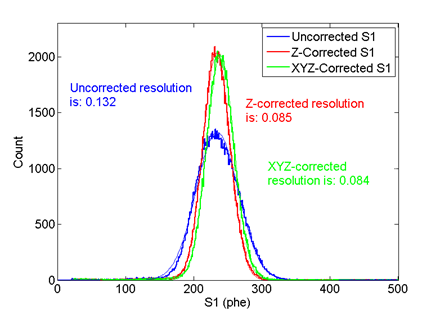
\includegraphics[scale=.75]{KRS1_ResolutionImprovement.png} 
\captionof{figure}{The $^{83m}$Kr S1 spectrum with no corrections applied (blue), z dependent corrections applied (red), and three dimensional xyz dependent corrections applied (green). Data from lux10\_20130510T1250.}
\label{KrS1Improvement}
\end{figure}

\begin{figure} [!h]
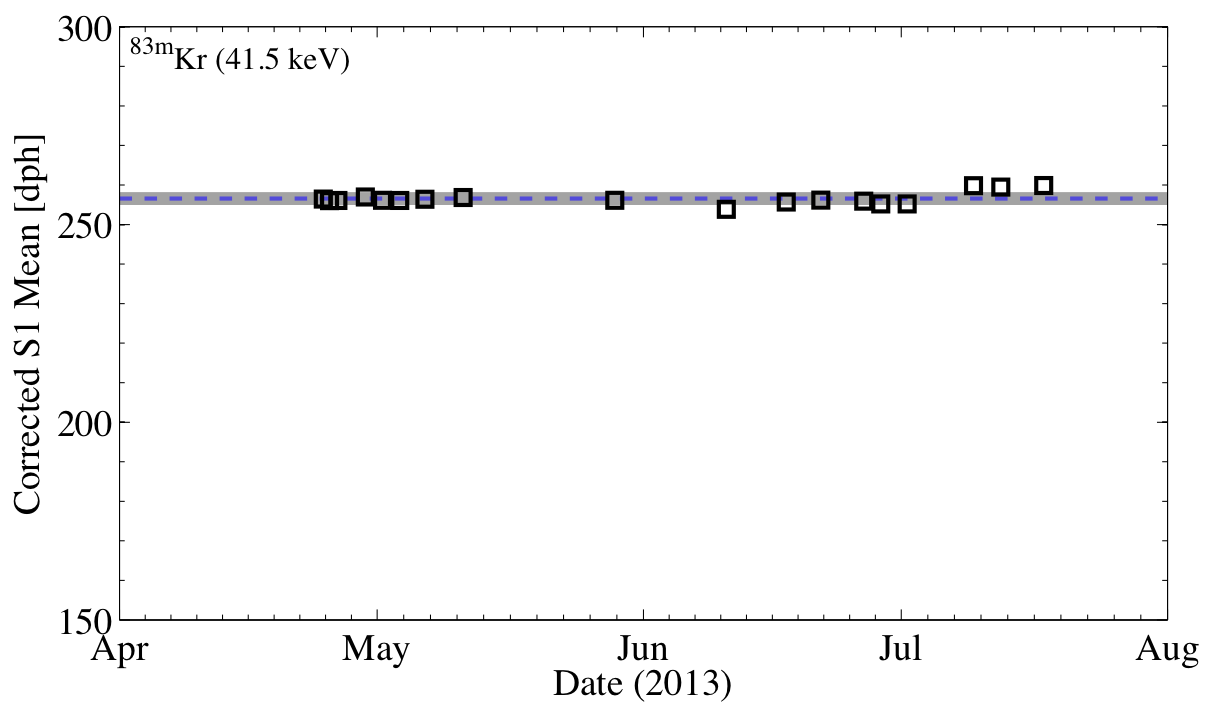
\includegraphics[scale=.35]{CorrectedS1_Stability.png} 
\captionof{figure}{The corrected $^{83m}$Kr S1 mean over the duration of LUX's Run03 data taking campaign. The dashed blue line indicates the mean of the corrected $^{83m}$Kr S1 spectrum over time, and the grey band indicates one standard deviation around the mean.}
\label{KrS1Stability}
\end{figure}

\subsection{S2 Corrections} \label{S2SignalCorr}

As with the S1 signal, we measure the Z dependence of the $^{83m}$Kr S2 pulse areas by slicing the detector into drift time bins with widths defined such that each bin has roughly 300 events.  Since the main source of drift time dependence in the S2 signal is the attenuation of charge due to electronegative impurities in the liquid xenon, an exponential decay is fit to the drift time dependence of the mean of each $^{83m}$Kr S2 distribution (Figure~\ref{fig:KrypCal_S2ZDep}).  A detector inefficiency correction for the Z direction is defined by taking the ratio of the S2  pulse area just below the liquid surface to the S2 pulse area as a function of Z as described in the equation
\begin{equation}
\mbox{S}2_{\mbox{z-efficiency-correction}} = \frac{S2(z=0)}{S2(z)}.
\end{equation} 

%Show S2 Gaussian fits and exponential fit here -- can probably get it from LUG
\begin{figure} 
\centering
\subfloat{{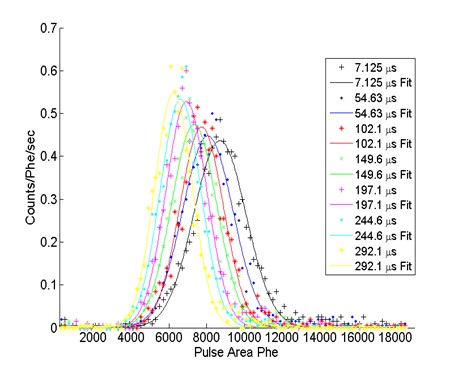
\includegraphics[width=6.3cm]{KrS2_ZDep_Gaussians.png} }}
\qquad
\subfloat{{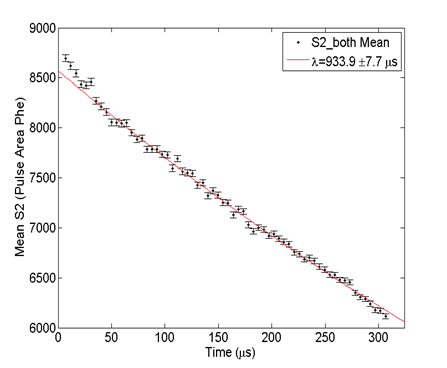
\includegraphics[width=6.3cm]{KrS2_ZDep.png} }}
\caption{ (Left) Gaussian distribution fits to $^{83m}$Kr S2 data that are used to determine the drift time dependence of the S2 pulse area. (Right) The z dependence of the S2 pulse area. Black points indicate the maximum of Gaussian distribution fits for each drift time bin, and red points indicate the exponential fit to that data. Data from lux10\_20130510T1250.}
\label{fig:KrypCal_S2ZDep}
\end{figure}

The process of measuring the XY dependence of the S2 signal is identical to the process of measuring the XY dependence of the S1 signal.  The z-corrected ($S2 \times \mbox{S}2_{\mbox{z-efficiency-correction}}$) S2 data is divided into two dimensional XY bins with areas defined such that each bin has roughly 300 events, and a Gaussian distribution is fit to the data of each bin.  The mean of the Gaussian distribution from each bin is used to construct S2 XY dependence maps, with a spline interpolation and extrapolation being used to determine the XY dependence between and outside of the bins. (Figure~\ref{fig:KrypCalS2XYDep}) A detector inefficiency correction for the XY direction is defined by taking the ratio of the z-corrected S2 pulse area at the center of the detector to the z-corrected S2 pulse area as a function of XY in cm, as shown below
\begin{align}
\mbox{S}2_{\mbox{xy-efficiency-correction}} &= \frac{\mbox{S}2_{\mbox{z-efficiency-correction}}\times S2(x_c,y_c,z)}{\mbox{S}2_{\mbox{z-efficiency-correction}}\times S2_(xyz)}.
\end{align} 
where $x_c$ and $y_c$ are the x and y center of the detector in uncorrected position coordinates. The corrected S2 pulse areas are produced by multiplying the raw, uncorrected S2 pulse areas by the XY and Z correction factors
\begin{equation}
\mbox{S}2_{\mbox{corrected}} = \mbox{S}2_{\mbox{raw}} \left( \mbox{S}2_{\mbox{z-efficiency-correction}} \right) \left( \mbox{S}2_{\mbox{xy-efficiency-correction}} \right).
\end{equation}

%Show S2 XY correction here
\begin{figure} 
\centering
\subfloat{{\includegraphics[width=6.3cm]{KrS2_XYDep.png} }}
\qquad
\subfloat{{\includegraphics[width=6.3cm]{KrS2_XYDep_Norm.png} }}
\caption{ (Left) Two dimensional map of the XY dependence in $^{83m}$Kr S2 data determined by fitting a Gaussian distribution to XY bins of the data and tracking the mean of each fit.(Right) Two dimensional map of the XY correction factor which is applied to z-corrected S2 data. Data from lux10\_20130510T1250.}
\label{fig:KrypCalS2XYDep}
\end{figure}

The z-dependence of the S2 signal is a function of the liquid xenon purity, which is in turn a function of the detector's purification efficiency, the detector's flow rate, and the emanation rate of impurities from detector components.  Note that circulation outages have an immediate impact on the purity of the liquid xenon, since the zirconium getter is unable to counteract the emanation of impurities and since the sudden shock to the detector can release impurities from otherwise harmless locations such as the weir reservoir.  As a result, the S2 correction maps vary significantly over time and must be remeasured on a weekly basis.

%Show lifetime plots from Run03 here
%\begin{figure} [!h]
%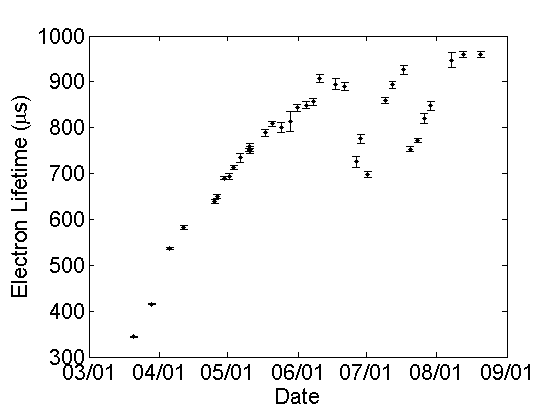
\includegraphics[scale=.75]{LUX_eLifetime_Run03.png} 
%\captionof{figure}{The electron lifetime over the duration of LUX's Run03 data taking campaign.}
%\label{KrS2Improvement}
%\end{figure}


\newpage

Figure~\ref{KrS2Improvement} shows the $^{83m}$Kr S2 spectrum from one particular data set before and after pulse area corrections are applied. In this data set the corrections improve the S2 resolution by 22\%, and shifts the mean by 21\%.  The large shift in the $^{83m}$Kr S2 mean is a result of the corrections "adding in" the electrons which were absorbed by impurities in the liquid xenon as they traveled to the surface.  Note that the resolution improvement and the shift of the mean are larger in data sets which have worse xenon purity.  As with the corrected S1 signal, the corrected S2 pulse areas are found to be extremely uniform over time, with the corrected $^{83m}$Kr S2 varying by less than 2\% over the course of the LUX detector's Run03 data taking campaign (Figure~\ref{KrS2Stability}).  Note that this reflects the fundamental stability of the anode and gas gain.  Only the liquid xenon purity seems to vary.

\begin{figure} [!h]
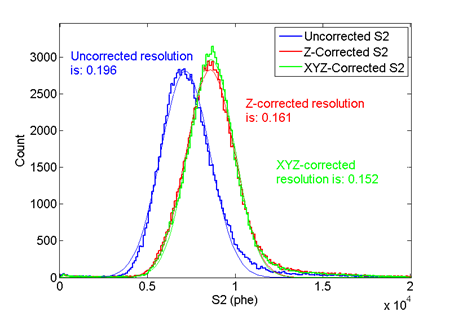
\includegraphics[scale=.7]{KRS2_ResolutionImprovement.png} 
\captionof{figure}{The $^{83m}$Kr S2 spectrum with no corrections applied (blue), z dependent corrections applied (red), and xyz dependent corrections applied (green). Data from lux10\_20130510T1250.}
\label{KrS2Improvement}
\end{figure}

\begin{figure} [!h]
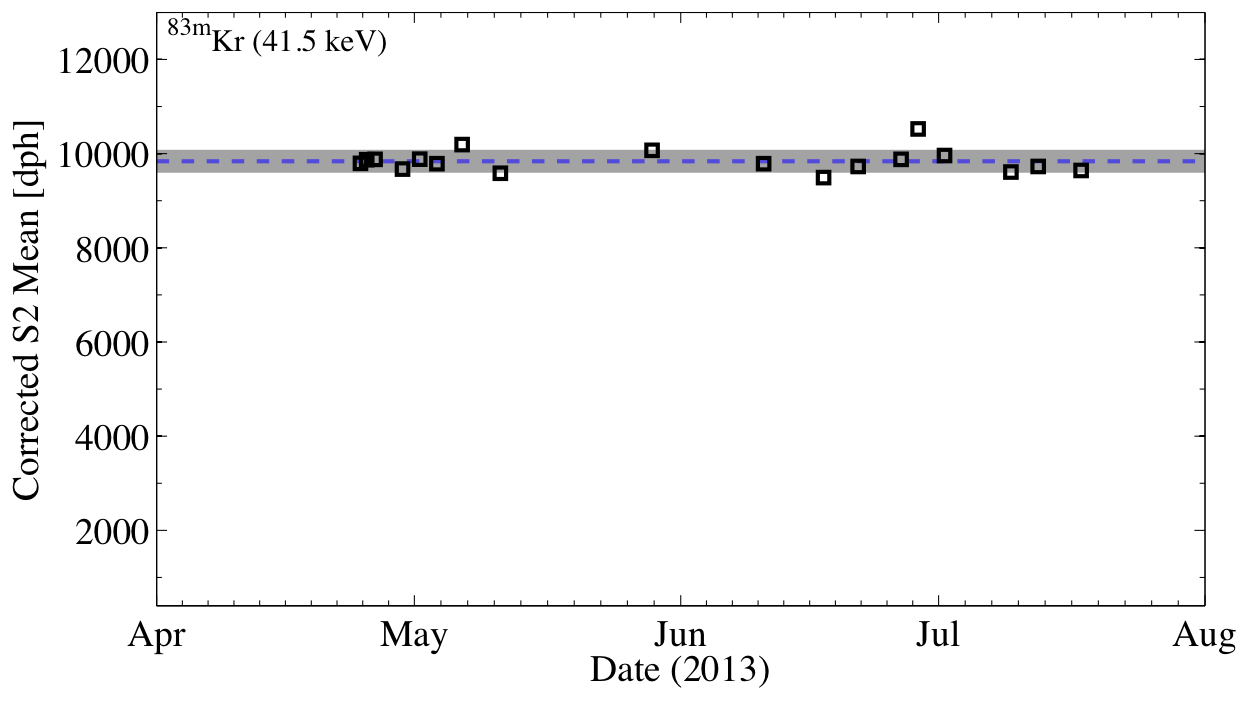
\includegraphics[scale=.3]{CorrectedS2_Stability.png} 
\captionof{figure}{The corrected $^{83m}$Kr S2 mean over the duration of LUX's Run03 data taking campaign.  The dashed blue line indicates the mean of the corrected $^{83m}$Kr S2 spectrum over time, and the grey band indicates one standard deviation around the mean.}
\label{KrS2Stability}
\end{figure}

\subsection{Future use of $^{83m}$Kr-Based Signal Corrections}

The previous sections described the primary techniques used during the LUX Run3 data analysis.  The monoenergetic peak of the $^{83m}$Kr calibration source provides a powerful tool to track signal variations throughout the detector, and the short half life allows for frequent calibration.  In the next generation of dark matter detectors, it's possible that $^{83m}$Kr's short half life will become a hindrance, since the source may not have time to mix uniformly throughout the larger detector volumes.  In this case, a longer lived calibration source, such as $^{131m}Xe$, may be used in a similar manner.  These more persistent sources must decay at a high energy to avoid contributing to the WIMP search backgrounds, leading to complications involving PMT saturation which are not present in the standard $^{83m}$Kr source.

In the following sections, we will describe a number of alternative signal correction techniques.  Although most of these additional methods were not used in the final Run3 analysis, they can improve the quality of future LUX analyses, and serve as a proof of concept for the next generation of dark matter detectors.

\subsection{Radon as a measure of Electron Lifetime}

The method of extracting electron lifetimes described in Section~\ref{S2SignalCorr} requires high statistics $^{83m}$Kr data sets for calibration.  While this method is reliable, data between an electron lifetime changing event, such as a circulation stop, and a $^{83m}$Kr calibration data set is unusable due to the lack of an electron lifetime measurement.  In this section we will discuss using $^{222}$Rn events to recover electron lifetime measurements from individual WIMP search data sets so that signals corrections can be applied even if a $^{83m}$Kr calibration is not available.

A few hundred Radon-222 appear in every LUX data set, with an observed rate of 17.9 $\pm$ 1.32 mHz in the active volume~\cite{BradleyThesis}.  While it is an unwanted background in the data, the Radon-222 alpha peak is useful for continuous monitoring of our electron lifetime.  Radon events are selected using a box cut on the raw S1 pulse areas.  An upper limit of 240 $\mu$seconds is placed on the drift time of selected events, since capacitor depletion causes the PMTs to saturate above this point (Figure~\ref{fig:RadonSelection}).  More precisely, when the observed signal exceeds $2.5\times10^4$ phe in an individual PMT, saturation becomes apparent, and the radon data becomes indistinguishable from the other alpha bands~\ref{LuxSaturation}.  The S1 pulse areas do not have a time dependence in Run3, so the same box cut is applicable to data at any point in time.  To ensure we are using clean radon data we only use the S2 signal from the bottoms PMT array to avoid PMT saturation.  After selection cuts are applied there are not enough radon events in a single data set to slice the detector into drift time bins as we did during $^{83m}$Kr calibrations.  Instead, we turn to a maximum likelihood approach to extract the electron lifetime from the limited amount of radon data.


\begin{figure}[h]\centering
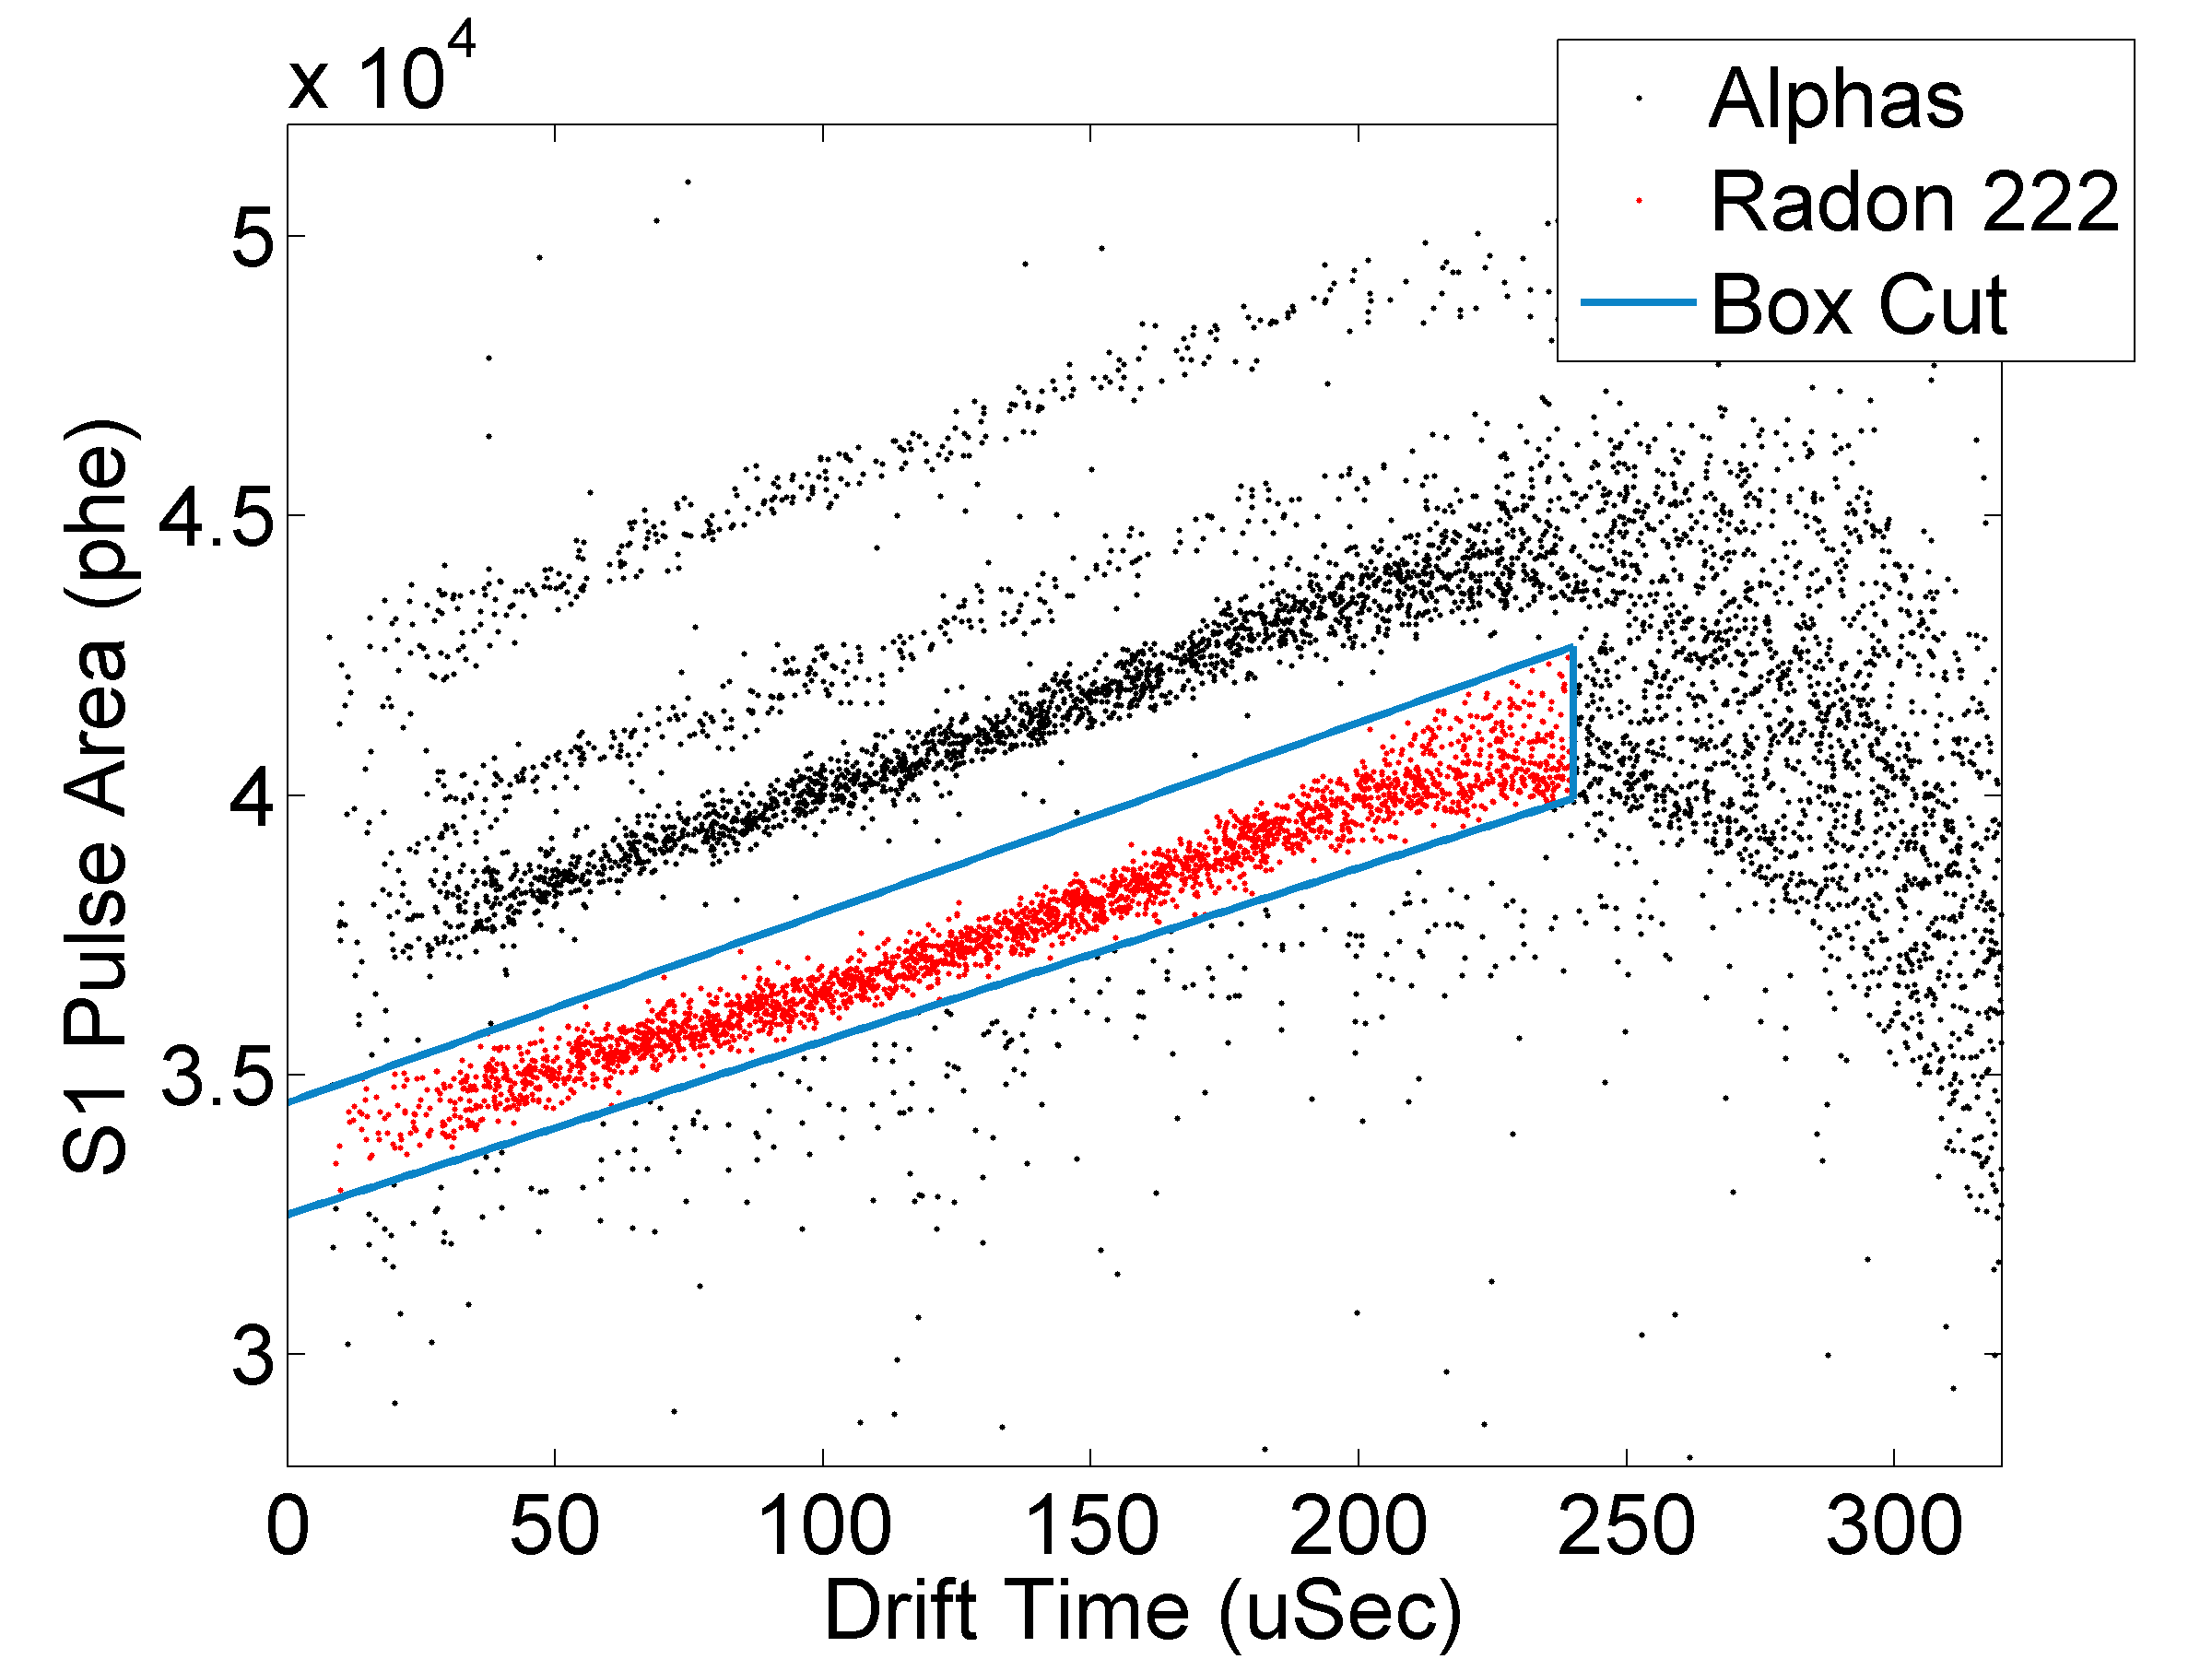
\includegraphics[scale=0.5]{RadonSelection.png}
\caption{Selection of radon events from a week of WIMP search data.  Black points include data from all alpha sources, and the blue lines indicate the box cut that is used to select $^{222}$Rn data (shown in red). At high drift times the S1 signals begin to saturate, leading to the turn over of events above 250 $\mu$seconds.}
\label{fig:RadonSelection}
\end{figure}

%Likelihood fitting described in: https://en.wikipedia.org/wiki/Maximum_likelihood
In the maximum likelihood analysis, a probability distribution function is used to determine the probability that an S2 of a given size and drift time will be measured, assuming some value for the electron lifetime.  There are two possible probability distribution functions which we can use.  The first PDF fits an attenuated Gaussian model to the attenuated S2 data, and is given by
\begin{equation}
\mbox{F}(x_i, z_i \text{\textbar} \mu, \sigma, \lambda) = \frac{1}{\sqrt{2\pi}\sigma} e^\frac{(-x_i - \mu e^\frac{-z_i}{\lambda})^2}{(2\sigma)^2}, 
\end{equation}
where $\sigma$ and $\mu$ are the Gaussian sigma and mean of the corrected radon peak based on the most recent krypton calibration data set, $x_i$ and $z_i$ are the uncorrected S2 and depth of the ith event in the data set, and $\lambda$ represents the unknown electron absorption length for the data set.  The second PDF fits a true Gaussian to the corrected S2 data, $x_i e^\frac{z_i}{\lambda}$, and is given by
\begin{equation}
\mbox{F}(x_i, z_i \text{\textbar} \mu, \sigma, \lambda) = \frac{1}{\sqrt{2 \pi} \sigma} e^\frac{(-x_i e^\frac{z_i}{\lambda} - \mu)^2}{(2 \sigma)^2}. 
\end{equation}
In either case, the PDF is evaluated for each event.  The likelihood of observing all of the events in a data set, for some value of $\mu$, $\sigma$, and $\lambda$ is then given by the likelihood function
\begin{equation}
\mathcal{L}(\mu, \sigma, \lambda ; x_i, z_i) = \prod_{i=1}^{n} F(x_i, z_i \text{\textbar} \mu, \sigma, \lambda)
\end{equation}
We wish to determine the electron lifetime value which has the highest likelihood of producing the observed data.  For convenience, we choose to minimize the negative of the log of the likelihood function with respect to $\lambda$, since it is less computationally expensive to minimize a summation than it is to maximize a product.  

After running the maximum likelihood method on all of the LUX detector's Run03 data sets we see that the attenuated Gaussian PDF is in better agreement with the z-slice method from Section~\ref{S2SignalCorr}. (Figure~\ref{fig:RadonLifetimeResults}) In either case, the results of the maximum likelihood fit from Radon data fall within one sigma of the results from $^{83m}$Kr calibrations. 

\begin{figure}[h]\centering
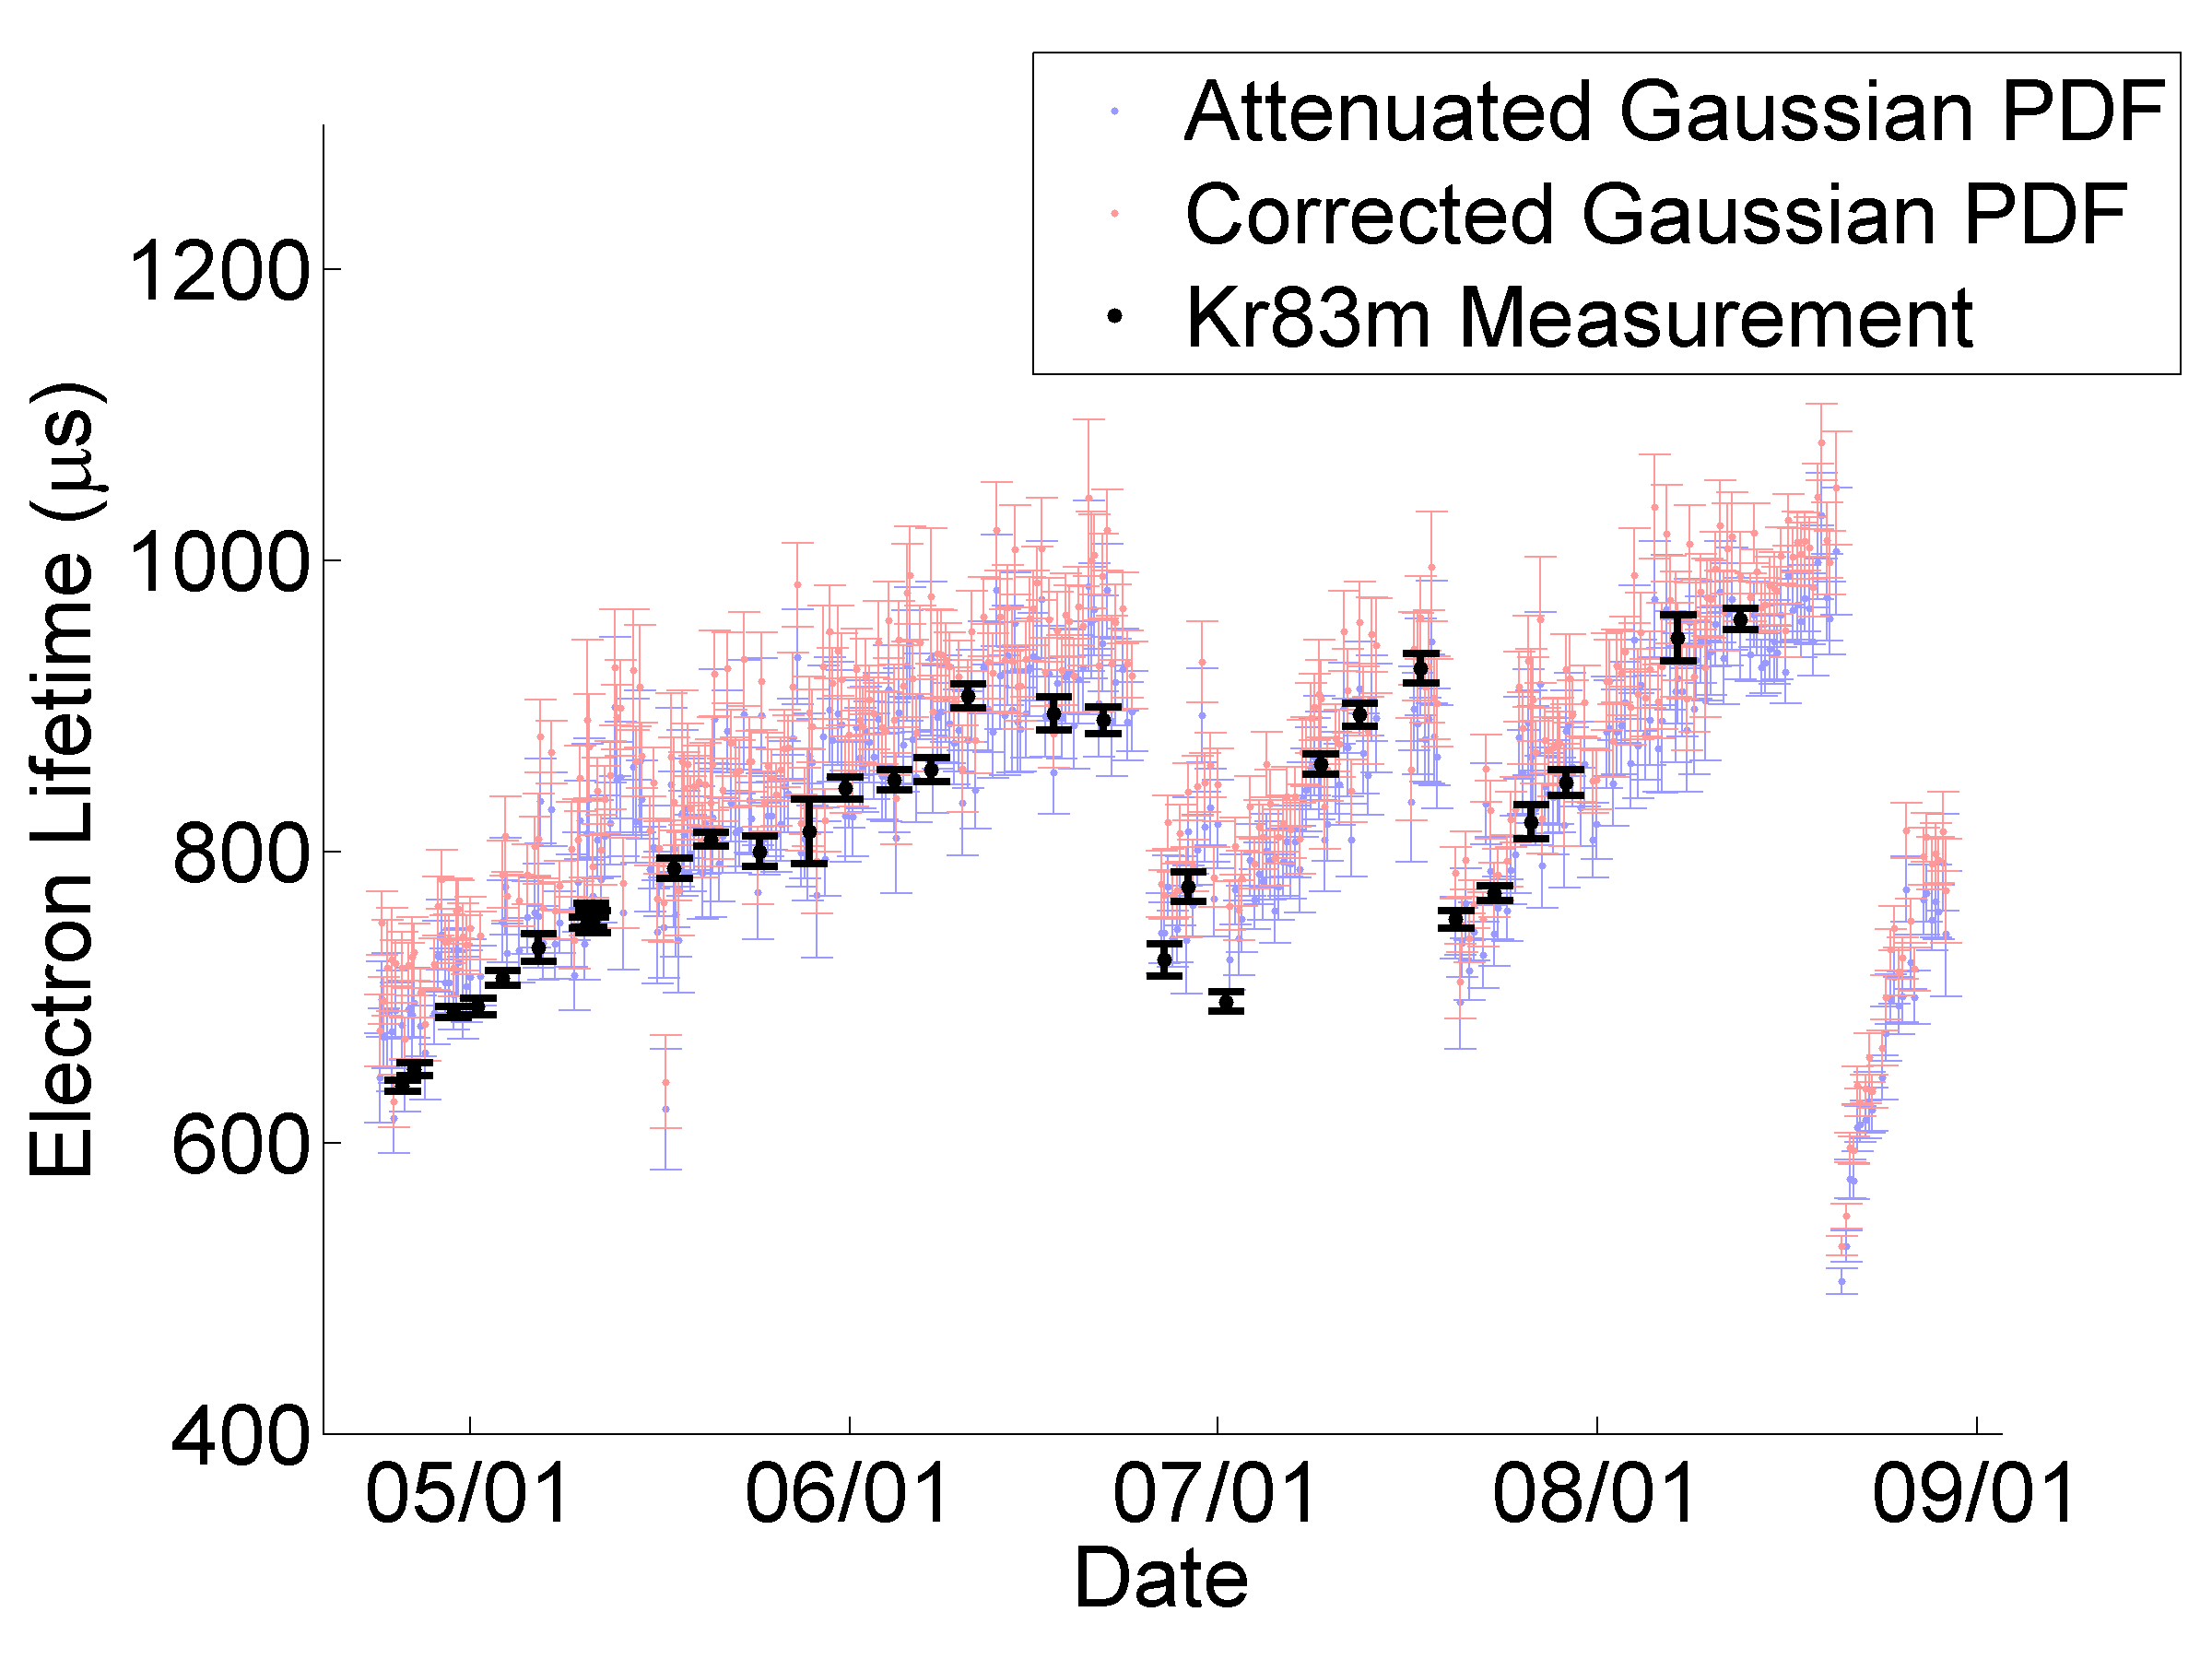
\includegraphics[scale=0.6]{RadonLifetimeResults.png}
\caption{A comparison of the calculated electron lifetimes based on the maximum likelihood method with an attenuated Gaussian PDF (in blue) and corrected Gaussian PDF (in red).  The electron lifetime measured from $^{83m}$Kr calibrations is shown in black.}
\label{fig:RadonLifetimeResults}
\end{figure}

The radon lifetime measurements described here are most useful following a circulation outage, since $^{83m}$Kr calibration data may not be available to measure any sudden drops in xenon purity.   Only two circulation stops occurred during LUX's Run3 data taking campaign, so the radon lifetime measurements only recovered a few days of livetime for the final Run3 analysis~\cite{Phelps}.  Circulation outages were far more common in LUX's Run4 data analysis, but complications from the non-uniform drift field at the time made the radon source a poor predictor of the detector's electron lifetime.  In particular, since most electrons recombine during an alpha interaction, small variations in the detector's electric field (and subsequentally the electron's recombination rate) result in large variations in radon S2 signal.  

LUX's successor, LZ, plans to use a persistent $^{131m}$Xe calibration source to produce signal corrections.  With an ever-present calibration source, it is unlikely that $^{222}$Rn would be used as more than a cross check of the standard electron lifetime measurements.  The stringent LZ backgrounds limits (less than 0.67 mHz of $^{222}$Rn activity) also make the techniques presented in this section less useful, since over 25 times the amount of data shown here would be needed to  produce similar precision.

 
\subsection{A PMT-by-PMT approach to S1 Corrections}

The S1 correction method presented in Section~\ref{S1SignalCorr} improves the detector's resolution by normalizing the summed S1 signal to the center of the detector.  While this method is used in the final LUX Run3 analysis, it is possible to improve the detector's S1 resolution further by defining a light collection map on a PMT-by-PMT basis~\cite{Akerib:2015rjg}.  For each S1 event we define the position corrected S1 signal using the weighted arithmetic mean of each PMT's spatially normalized S1 measurement, given by
\begin{equation} \label{WeightedMean}
S1_{\mbox{corrected}} = \frac{\sum_{j=1}^{j=122} S1^{\prime}_{j} W_{j}} {\sum_{j=1}^{j=122} W_{j}},
\end{equation}
where $S1^{\prime}_{j}$ is the spatially normalized S1 signal of the $j$th PMT and $W_j$ is the weight given to $j$th PMT's measurement.

Since we want the corrected S1 signal to be spatially uniform, the spatially normalized S1 signal for each PMT is given by
\begin{equation}
S1^{\prime}_{j} = S1_{\mbox{sc}} \frac{S1_j}{\langle S1 \rangle_{j}}
\end{equation}
where $S1_{\mbox{sc}}$ is the summed $^{83m}$Kr S1 signal at the center of the detector, $S1_j$ is the S1 signal of the $j$th PMT, and $\langle S1 \rangle_{j}$ is the average $^{83m}$Kr S1 signal recorded in the vicinity of the S1 event by the $j$th PMT.  It is useful to think of the $ \frac{S1_j}{\langle S1 \rangle_{j}}$ term as measuring the strength of the $S1_j$ signal as a fraction of the average $^{83m}$Kr $S1_j$ signal, and the $S1_{\mbox{sc}}$ term as a normalization constant which scales the fractional signal to the equivalent $S1$ size at the center of the detector.

The weights of the arithmetic mean are given by relative variance of each PMT's measurement,
\begin{equation}
W_j=\frac{{\langle S1 \rangle_{j}}^2}{\sigma_j^2},
\end{equation}
where $\sigma_j^2$ is the variance of the S1 signal in $j$th PMT in the vicinity of the event.  It is important to use the relative variance of each PMT for the weights, since the absolute variance grows larger with the size of the S1 signal and would therefore give lower weight to PMTs which observe a stronger S1 signal.  Equation~\ref{WeightedMean} then becomes
\begin{equation} \label{WeightedMean2}
S1_{\mbox{corrected}} = S1_{\mbox{sc}} \frac{\sum_{j=1}^{j=122} \frac{S1_j}{\langle S1 \rangle_{j}} \frac{{\langle S1 \rangle_{j}^2}}{\sigma_j^2}} {\sum_{j=1}^{j=122} \frac{{\langle S1 \rangle_{j}}^2}{\sigma_j^2}}.
\end{equation}

It is difficult to measure the relative variance of the $j$th PMT at all points in the detector, since doing so involves interpolating small values from two different three dimensional maps of  $\sigma_j^2$ and $\langle S1 \rangle_{j}$.  Instead, we can achieve the same result by normalizing the S1$j$ signal to the value of S1$_{\mbox{sc}}$ prior to calculating the arithmetic mean.  In this case, the normalized S1$_{\text{N},j}$ signal is calculated by scaling the raw S1$_j$ signal by a normalization factor
\begin{equation}
S1_{\text{N},j}=\frac{S1_{\mbox{sc}}}{\langle S1 \rangle_{j}} S1_j.
\end{equation}
Consequently, the standard deviation and mean of the S1$j$ signal are scaled by the same factor, such that
\begin{equation}
\sigma_{\text{N},j} = \frac{S1_{\mbox{sc}}}{\langle S1 \rangle_{j}} \sigma_j
\end{equation}
\begin{equation}
\langle S1 \rangle_{\text{N},j} = \frac{S1_{\mbox{sc}}}{\langle S1 \rangle_{j}} \langle S1 \rangle_{j} = S1_{\mbox{sc}}.
\end{equation}
Using the normalized $S1_{\text{N},j}$ signal, Equation~\ref{WeightedMean2} becomes
\begin{equation} \label{WeightedMean3}
S1_{\mbox{corrected}} = S1_{\mbox{sc}} \frac{\sum_{j=1}^{j=122} \frac{S1_{\text{N},j}}{\langle S1_{\text{N},j} \rangle}\frac{1}{ \sigma_{\text{N},j}^2}}{ \sum_{j=1}^{j=122} \frac{1}{\sigma_{\text{N},j}^2}}
\end{equation}
In practice, Equation~\ref{WeightedMean3} is easier to implement and more accurate than Equation~\ref{WeightedMean2}, since it requires fewer interpolations of the mean and variance maps from the $^{83m}$Kr data.

It is worth noting that if the S1$_j$ distributions are Poissonian, Equation~\ref{WeightedMean2} (and Equation~\ref{WeightedMean3}) reduces to the S1 correction method described in Section~\ref{S1SignalCorr}.  In this case 
\begin{equation}
\sigma_{j}^2 = \langle S1 \rangle_{j}
\end{equation}
so Equation~\ref{WeightedMean2} becomes
\begin{equation}
S1_{\mbox{corrected}} = S1_{\mbox{sc}} \frac{\sum_{j=1}^{j=122} S1_j}{\sum_{j=1}^{j=122} \langle S1 \rangle_{j}} = S1_{\mbox{sc}} \frac{S1}{\langle S1 \rangle}
\end{equation}
Where $S1$ is the sum of all of the PMT signals for the event and $\langle S1 \rangle$ is the average of the sum of the PMT signals for $^{83m}$Kr events. Therefore, this PMT-by-PMT method is only beneficial if significant non-Poissonian noise is present in the PMT signals.

Figure~\ref{PMTxPMTResult} shows the result of applying the PMT-by-PMT method to the lux10\_20130510T1250 $^{83m}$Kr data set.  Within the fiducial volume the resolution of the S1 signal improves by 13\% over the standard correction method from section~\ref{S1SignalCorr}.  Outside of the fiducial volume, the interpolations of the variance and mean maps become extrapolations.  This leads to significant inaccuracies in the weighted mean measurement, causing non-Gaussian tails to appear in the S1 distribution.  Therefore, for events within the fiducial volume the PMT-by-PMT method is an improvement over the standard correction method, but for events outside of the fiducial volume the less complex standard correction method is ideal.


\begin{figure} [h!]
\centering
\subfloat{{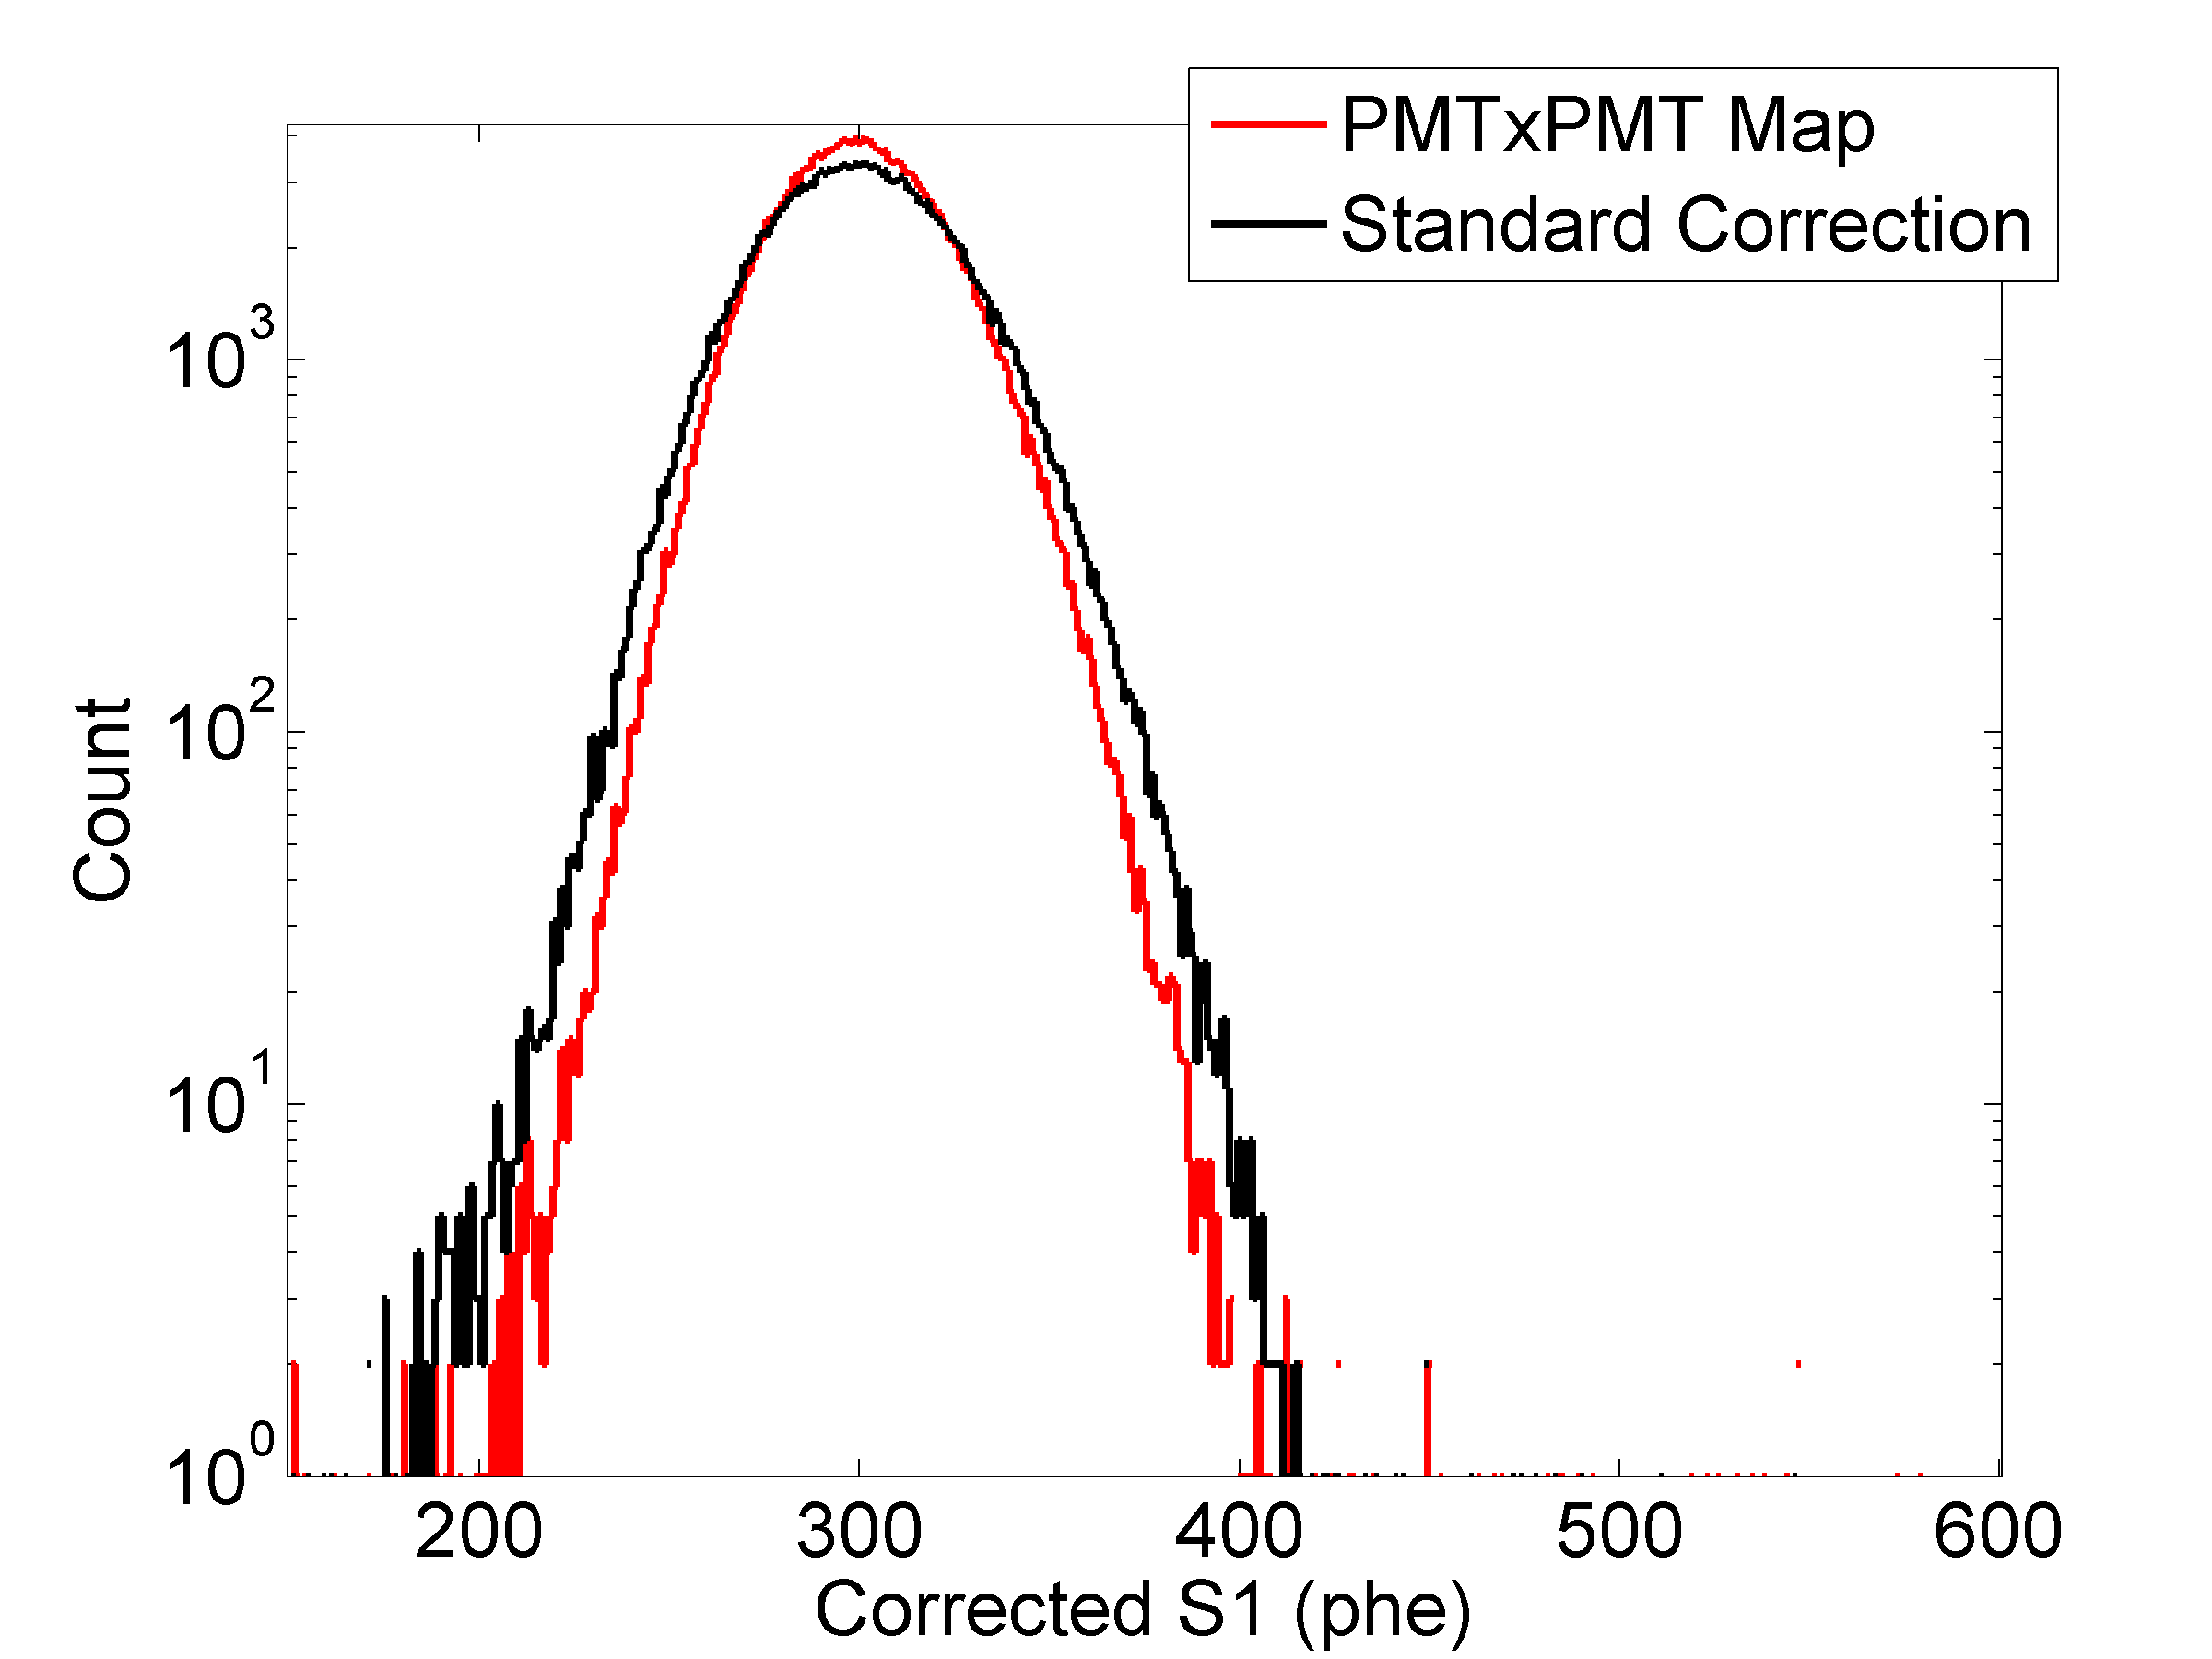
\includegraphics[width=6.3cm]{PMTxPMT_Fiducial_logy.png} }}
\qquad
\subfloat{{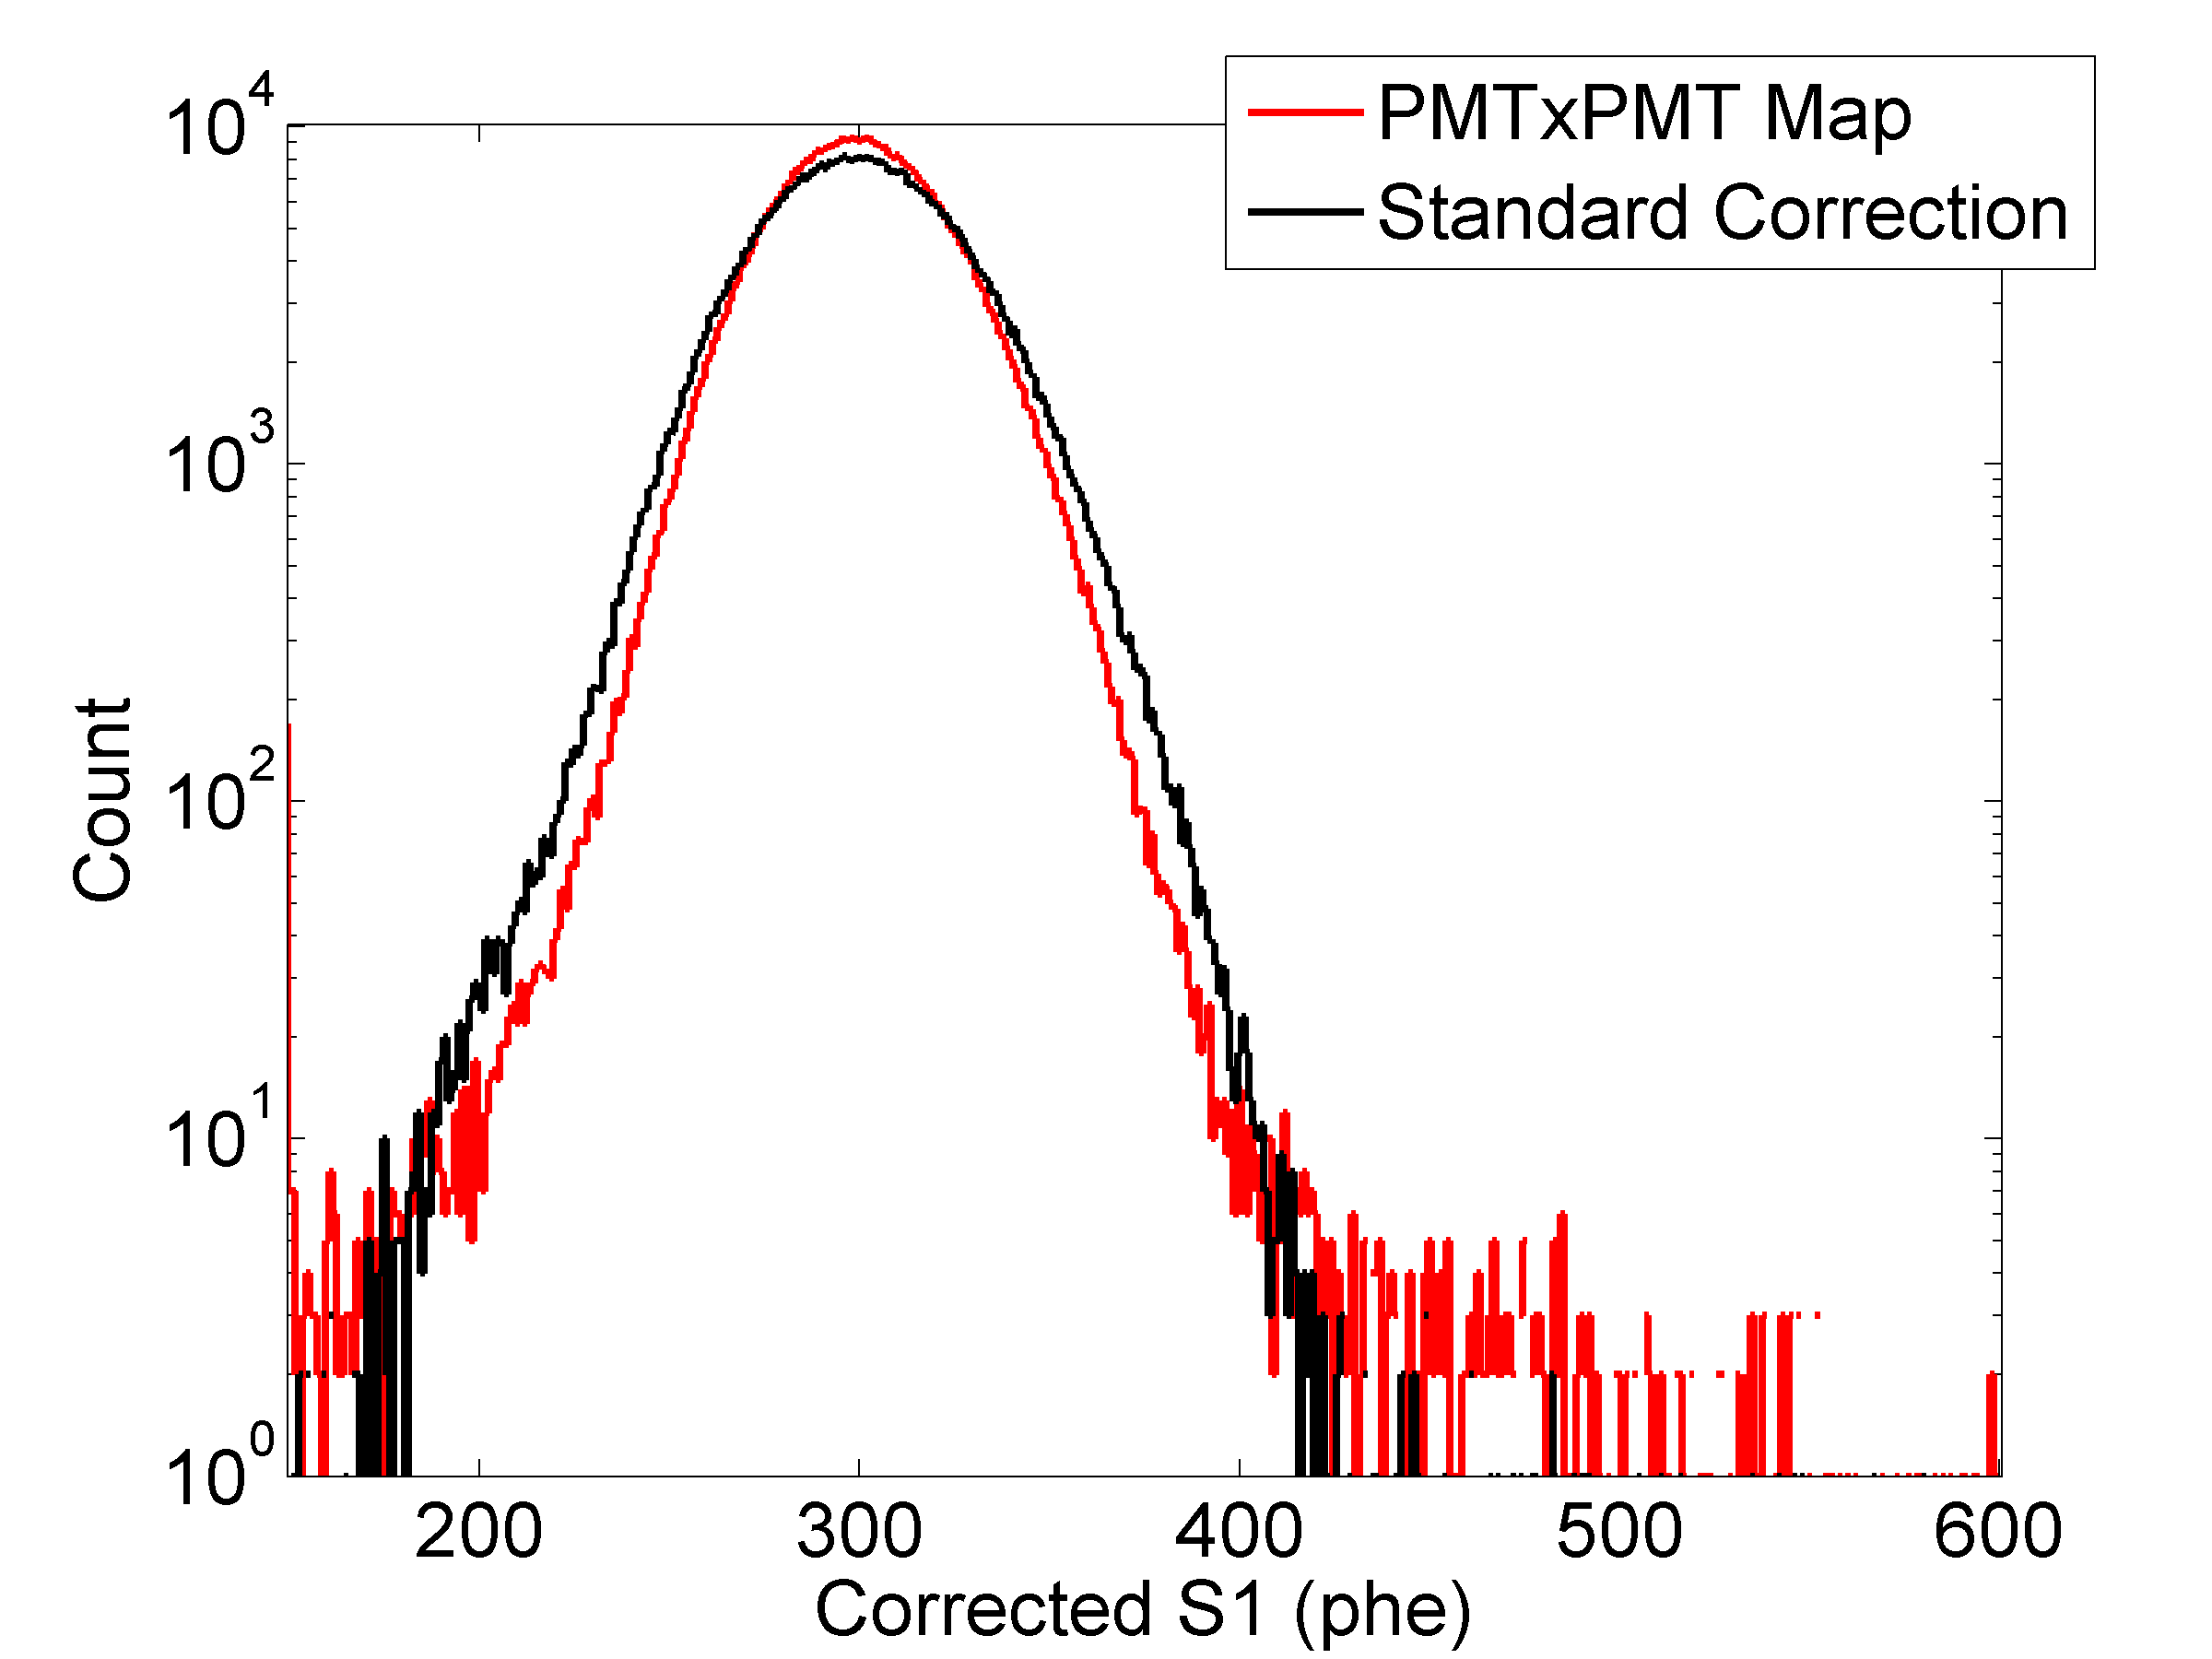
\includegraphics[width=6.3cm]{PMTxPMT_NoFiducial_logy.png} }}
\caption{ The $^{83m}$Kr corrected S1 spectrum after applying the PMT-by-PMT method (in red) and after applying the standard correction method from Section~\ref{S1SignalCorr} (in black).  The events within the fiducial volume are shown on the left, and all of the events are shown on the right.}
\label{PMTxPMTResult}
\end{figure}

The techniques presented in this section were never used in published LUX results.  Although the results show moderate improvement in the detector's resolution, they do not produce an equally impactful improvement in the final WIMP search limits. (This is because the detector's background models have a larger impact than the detector's energy resolution in the profile likelihood analysis.)  Therefore, since these methods require significant computing power to implement, there was little motivation to include them in the final corrections module.  Future LUX analyses, such as a search for sterile neutrinos, may benefit more from an improved detector resolution, at which point it may be worthwhile to implement the techniques described here.

\subsection{Signal Corrections Summary}

In this chapter, we discussed the standard techniques that were used to produce signal corrections in LUX's Run3 data.  The most impactful methods centered around $^{83m}$Kr data, due to the usefulness of the source's short lived monoenergetic signal.  We also discussed two alternative correction methods, which did not have a signficant impact on the current LUX analysis, but may be useful in future.  In Chapter~\ref{Run04Corrections}, we'll find that the non-uniform Run4 drift field introduces signifanct complications to the $^{83m}$Kr data, which must be accounted for before the methods of this chapter can be applied to that data.  